\section{Appendix}

\subsection{Matlab version}
\lstset{language=Matlab, caption={Lattice Boltzmann Model, implemented in Matlab},label=lbmmatlab, captionpos=t}
\lstinputlisting{./code/lbm2d.m}

\newpage
\subsection{NumPy version}
\lstset{language=Python, caption={Lattice Boltzmann Model, implemented in NumPy},label=lbmnumpy}
\lstinputlisting{./code/lbm2d.py}

\newpage
\subsection{PyCUDA version}
\lstset{language=Python, caption={Lattice Boltzmann Model, implemented in PyCUDA},label=lbmcuda}
\lstinputlisting{./code/lbm2dcu.py}


\subsection{Results}
\begin{table}[H]
\centering
\begin{tabular}{lllll}
\toprule
Size	 of field &1st run(s)&	2nd run(s)&	3rd run(s) &	Average(s)\\
\midrule
16&	0.746133&	0.734992&	0.734949&	0.738691333\\
32&	1.246536&	1.233322&	1.240871&	1.240243\\
48&	2.071759&	2.061449&	2.050736&	2.061314667\\
64&	3.16993&		3.206161&	3.247185&	3.207758667\\
80&	4.73842&		4.636399&	4.638702&	4.671173667\\
96&	6.677765&	6.670117&	6.651408&	6.66643\\
112&	8.934494&	8.932387&	8.935797&	8.934226\\
128&	13.595282&	13.008162&	13.004377&	13.202607\\
144&	16.673446&	16.704629&	16.703753&	16.69394267\\
160&	21.004205&	21.109045&	21.096003&	21.069751\\
176&	25.085424&	25.239326&	25.256939&	25.19389633\\
192&	30.056787&	30.267888&	30.364107&	30.229594\\
208&	35.587349&	35.763984&	35.783916&	35.71174967\\
\bottomrule
\end{tabular}
\caption{Results from running the CPU-version of D2Q9 LBM, after 1000 iterations in an open channel scenery (\autoref{tunnelimages}). The simulated field is the independent variable, and the running time is the dependent variable.}
\label{resultcpu}
\end{table}


\begin{table}[H]
\centering
\begin{tabular}{lllll}
\toprule
Size	 of field &1st run(s)&	2nd run(s)&	3rd run(s) &	Average(s)\\
\midrule
16&	0.241659&	0.23915&		0.205136	&	0.228648333\\
32&	0.228573	&	0.285473&	0.234809	&	0.249618333\\
48&	0.351229	&	0.346322	&	0.378153	&	0.358568\\
64&	0.478636	&	0.479583	&	0.473222	&	0.477147\\
80&	0.647089	&	0.643426	&	0.67618	&	0.655565\\
96&	0.858993	&	0.879635	&	0.880193	&	0.872940333\\
112&	1.110316	&	1.106407	&	1.105429	&	1.107384\\
128&	1.410813	&	1.423374	&	1.387333	&	1.407173333\\
144&	1.696993	&	1.699721	&	1.692255	&	1.696323\\
160&	2.097632	&	2.072039	&	2.058629	&	2.0761\\
176&	2.503845	&	2.421257	&	2.425955	&	2.450352333\\
192&	2.779791	&	2.788359	&	2.759723	&	2.775957667\\
208&	3.440834	&	3.096601	&	3.096115	&	3.211183333\\
224&	3.668249	&	3.554599	&	3.534036	&	3.585628\\
240&	3.987397	&	3.989254	&	3.929123	&	3.968591333\\
256&	4.670454	&	4.484278	&	4.487079	&	4.547270333\\
272&	5.450173	&	5.123512	&	5.125534	&	5.233073\\
288&	5.666375	&	5.557551	&	5.555653	&	5.593193\\
304&	6.105622	&	6.097763	&	6.093172	&	6.098852333\\
320&	7.188123	&	6.79385	&	6.772588	&	6.918187\\
336&	7.328069	&	7.337078	&	7.309121	&	7.324756\\
352&	8.69325	&	7.965098	&	7.955409	&	8.204585667\\
368&	8.846718	&	8.673317	&	8.643207	&	8.721080667\\
384&	9.700574	&	9.562544	&	9.480546	&	9.581221333\\
400&	10.36871	&	9.965424	&	9.997083	&	10.11040567\\
416&	10.780117&	10.691381&	10.677279&	10.716259\\
432&	11.450054&	11.370197&	11.378999&	11.39975\\
448&	12.519018&	12.172332&	12.169165&	12.28683833\\
464&	13.893501&	13.025537&	13.011743&	13.31026033\\
480&	14.708758&	13.912262&	13.918446&	14.179822\\
496&	15.270144&	14.979782&	14.942925&	15.06428367\\
512&	16.212768&	15.585513&	15.59956	&	15.79928033\\
\bottomrule
\end{tabular}
\caption{Results from running the GPU-version of D2Q9 LBM, after 1000 iterations in an open channel scenery (\autoref{tunnelimages}). The simulated field is the independent variable, and the running time is the dependent variable.}
\label{resultgpu}
\end{table}

\subsection{Images}
\begin{figure}[H]
\centering
\subfigure[Open channel simulation calculated by PyCUDA]{
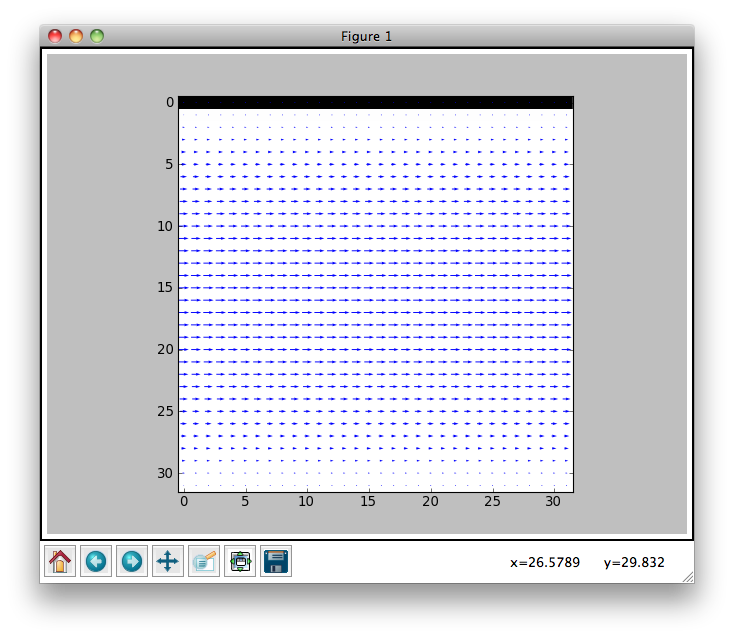
\includegraphics[width=0.47\textwidth]{./images/cuda_tunnel_32_32_900.png}
\label{tunnel}
}
\hspace{1pt}
\subfigure[The same simulation as in \autoref{tunnel} but with color gradient]{
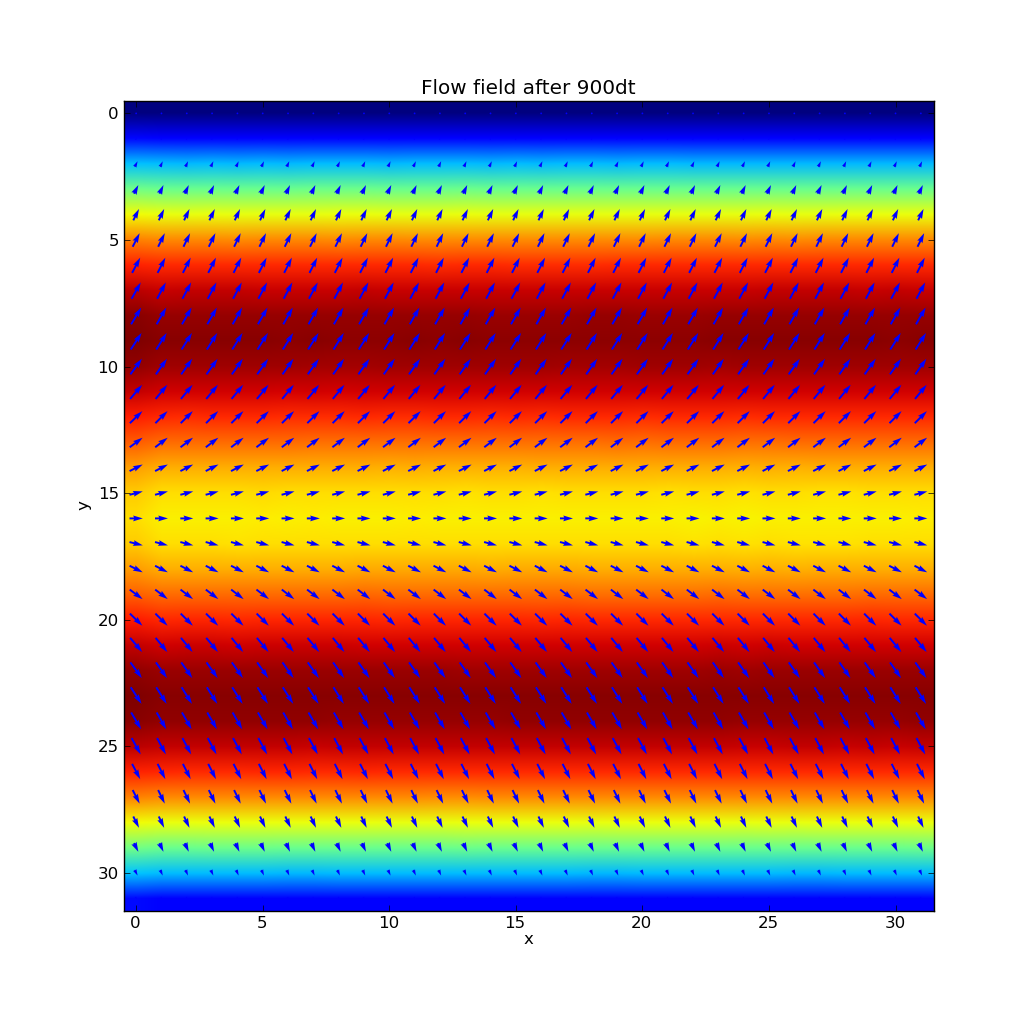
\includegraphics[width=0.47\textwidth]{./images/cuda_tunnel_32_32_900_color.png}
\label{tunnelcolor}
}
\caption{Open channel simulation, the simplest simulation used for verifying correctness of the simulation, as well as benchmarking the CPU- and GPU-version}
\label{tunnelimages}
\end{figure}